\documentclass[tikz]{standalone}
\usepackage{varwidth}
\usetikzlibrary{chains}
\begin{document}
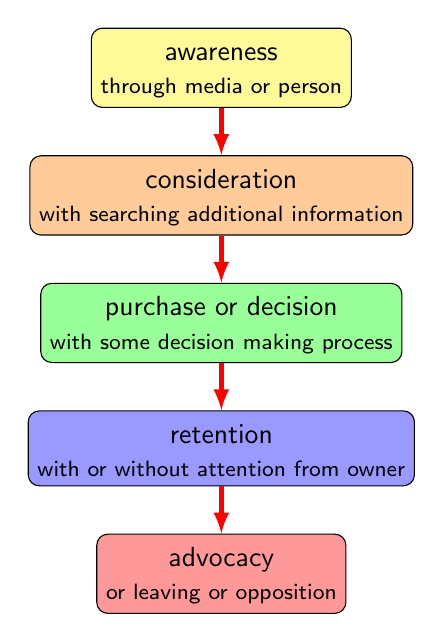
\begin{tikzpicture}[
    start chain=going below, node distance=6mm,
    every join/.style={->,>=latex, red, ultra thick},
    mynode/.style={
        rounded corners, draw, font=\sffamily,
        on chain, join,
        execute at begin node={\begin{varwidth}{5cm}\centering},
        execute at end node={\end{varwidth}}
    }
]
\foreach \mystep/\myexpl/\mycol in 
    {awareness/through media or person/yellow!40, 
    consideration/with searching additional information/orange!40,
    purchase or decision/with some decision making process/green!40,
    retention/with or without attention from owner/blue!40, 
    advocacy/or leaving or opposition/red!40
    }
    \node[mynode,fill=\mycol] {\strut\mystep\\\footnotesize\myexpl};
\end{tikzpicture}
\end{document}